\documentclass[tikz,border=12pt]{standalone}
\usepackage[T1]{fontenc}
\usepackage{mathpazo}
\usepackage{amsmath,amssymb}
\usetikzlibrary{arrows.meta, positioning, calc, patterns}

\definecolor{stblue}{HTML}{7B97AD}
\definecolor{rwgold}{HTML}{B8995E}
\definecolor{sage}{HTML}{7A9A7E}
\definecolor{dkbrown}{HTML}{3D3530}
\definecolor{wmgray}{HTML}{7B7067}
\definecolor{cream}{HTML}{F9F6F0}
\definecolor{border}{HTML}{D4C9B8}
\definecolor{terracotta}{HTML}{C47A6A}
\definecolor{lavender}{HTML}{907EA0}

\begin{document}
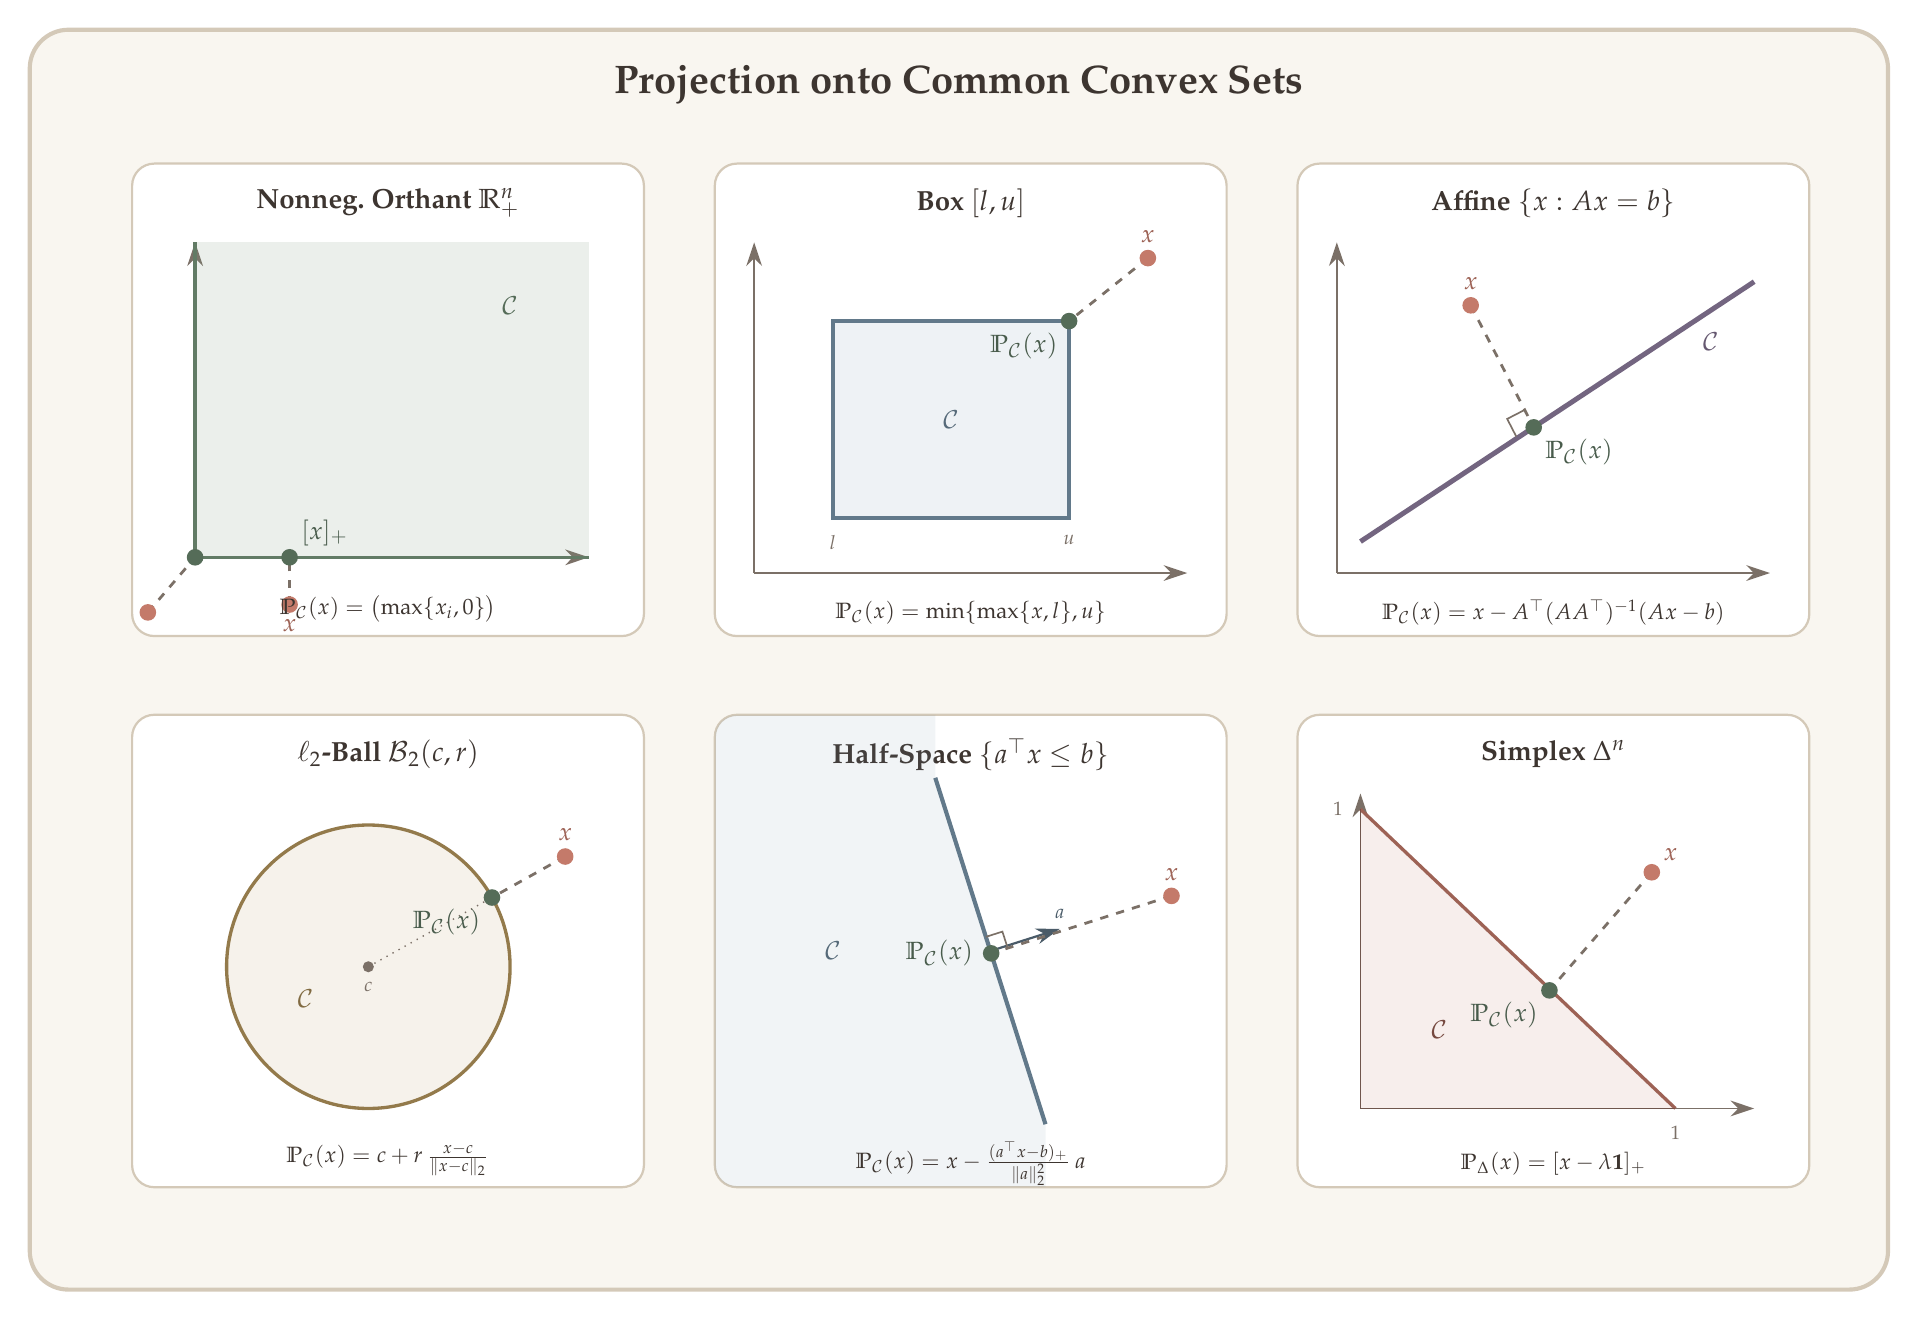
\begin{tikzpicture}[>={Stealth[length=3mm, width=2mm]}]

% Overall background
\fill[cream, rounded corners=14pt] (-0.8,-0.8) rectangle (22.8,15.2);
\draw[border, line width=1.5pt, rounded corners=14pt] (-0.8,-0.8) rectangle (22.8,15.2);

% Title
\node[text=dkbrown, font=\Large\bfseries] at (11,14.5)
  {Projection onto Common Convex Sets};

% Panel dimensions: each panel is roughly 6.5 wide x 6 tall
% Row 1: y offset = 7.5,  Row 2: y offset = 0.5
% Col 1: x offset = 0.5,  Col 2: x offset = 7.9,  Col 3: x offset = 15.3

% ============================================================
% Panel 1: Nonnegative Orthant (top-left)
% ============================================================
\begin{scope}[shift={(0.5,7.5)}]
  % Panel background
  \fill[white, rounded corners=8pt] (0,0) rectangle (6.5,6);
  \draw[border, line width=0.8pt, rounded corners=8pt] (0,0) rectangle (6.5,6);

  % Panel title
  \node[text=dkbrown, font=\bfseries] at (3.25,5.5) {Nonneg.\ Orthant $\mathbb{R}_+^n$};

  % Axes
  \draw[wmgray, line width=0.6pt, ->] (0.8,1.0) -- (5.8,1.0);
  \draw[wmgray, line width=0.6pt, ->] (0.8,1.0) -- (0.8,5.0);

  % Shaded first quadrant
  \fill[sage, opacity=0.15] (0.8,1.0) rectangle (5.8,5.0);
  \draw[sage!80!black, line width=1.2pt] (0.8,1.0) -- (5.8,1.0);
  \draw[sage!80!black, line width=1.2pt] (0.8,1.0) -- (0.8,5.0);

  % Label C
  \node[text=sage!70!black, font=\small\bfseries] at (4.8,4.2) {$\mathcal{C}$};

  % Point x outside (negative coordinates)
  \coordinate (x1) at (2.0,0.4);
  \coordinate (p1) at (2.0,1.0);

  % Dashed projection line
  \draw[wmgray, line width=1pt, dashed] (x1) -- (p1);

  % Points
  \fill[terracotta] (x1) circle (3pt);
  \node[text=terracotta!80!black, font=\small, below=2pt] at (x1) {$x$};
  \fill[sage!70!black] (p1) circle (3pt);
  \node[text=sage!60!black, font=\small, above right=1pt] at (p1) {$[x]_+$};

  % Another point outside (both coords negative)
  \coordinate (x1b) at (0.2,0.3);
  \coordinate (p1b) at (0.8,1.0);
  \draw[wmgray, line width=1pt, dashed] (x1b) -- (p1b);
  \fill[terracotta] (x1b) circle (3pt);
  \fill[sage!70!black] (p1b) circle (3pt);

  % Formula
  \node[text=dkbrown, font=\footnotesize] at (3.25,0.35)
    {$\mathbb{P}_{\mathcal{C}}(x) = \bigl(\max\{x_i,0\}\bigr)$};
\end{scope}

% ============================================================
% Panel 2: Box Constraints (top-center)
% ============================================================
\begin{scope}[shift={(7.9,7.5)}]
  \fill[white, rounded corners=8pt] (0,0) rectangle (6.5,6);
  \draw[border, line width=0.8pt, rounded corners=8pt] (0,0) rectangle (6.5,6);

  \node[text=dkbrown, font=\bfseries] at (3.25,5.5) {Box $[l,u]$};

  % Axes
  \draw[wmgray, line width=0.6pt, ->] (0.5,0.8) -- (6.0,0.8);
  \draw[wmgray, line width=0.6pt, ->] (0.5,0.8) -- (0.5,5.0);

  % Box region
  \fill[stblue, opacity=0.12] (1.5,1.5) rectangle (4.5,4.0);
  \draw[stblue!80!black, line width=1.2pt] (1.5,1.5) rectangle (4.5,4.0);

  \node[text=stblue!70!black, font=\small\bfseries] at (3.0,2.75) {$\mathcal{C}$};

  % Tick labels
  \node[text=wmgray, font=\scriptsize, below] at (1.5,1.4) {$l$};
  \node[text=wmgray, font=\scriptsize, below] at (4.5,1.4) {$u$};

  % Point outside, projected to corner
  \coordinate (x2) at (5.5,4.8);
  \coordinate (p2) at (4.5,4.0);
  \draw[wmgray, line width=1pt, dashed] (x2) -- (p2);
  \fill[terracotta] (x2) circle (3pt);
  \node[text=terracotta!80!black, font=\small, above=2pt] at (x2) {$x$};
  \fill[sage!70!black] (p2) circle (3pt);
  \node[text=sage!60!black, font=\small, below left=1pt] at (p2) {$\mathbb{P}_{\mathcal{C}}(x)$};

  % Formula
  \node[text=dkbrown, font=\footnotesize] at (3.25,0.3)
    {$\mathbb{P}_{\mathcal{C}}(x) = \min\{\max\{x,l\},u\}$};
\end{scope}

% ============================================================
% Panel 3: Affine Set (top-right)
% ============================================================
\begin{scope}[shift={(15.3,7.5)}]
  \fill[white, rounded corners=8pt] (0,0) rectangle (6.5,6);
  \draw[border, line width=0.8pt, rounded corners=8pt] (0,0) rectangle (6.5,6);

  \node[text=dkbrown, font=\bfseries] at (3.25,5.5) {Affine $\{x: Ax=b\}$};

  % Axes
  \draw[wmgray, line width=0.6pt, ->] (0.5,0.8) -- (6.0,0.8);
  \draw[wmgray, line width=0.6pt, ->] (0.5,0.8) -- (0.5,5.0);

  % Affine line
  \draw[lavender!80!black, line width=1.8pt] (0.8,1.2) -- (5.8,4.5);
  \node[text=lavender!70!black, font=\small\bfseries, below right=1pt] at (5.0,4.0) {$\mathcal{C}$};

  % Point and perpendicular projection
  \coordinate (x3) at (2.2,4.2);
  \coordinate (p3) at (3.0,2.65);
  \draw[wmgray, line width=1pt, dashed] (x3) -- (p3);
  \fill[terracotta] (x3) circle (3pt);
  \node[text=terracotta!80!black, font=\small, above=2pt] at (x3) {$x$};
  \fill[sage!70!black] (p3) circle (3pt);
  \node[text=sage!60!black, font=\small, below right=1pt] at (p3) {$\mathbb{P}_{\mathcal{C}}(x)$};

  % Right angle mark
  \coordinate (ra1) at ($(p3)!0.25cm!(x3)$);
  \coordinate (ra2) at ($(p3)!0.25cm!90:(x3)$);
  \coordinate (ra3) at ($(ra1)+(ra2)-(p3)$);
  \draw[wmgray, line width=0.6pt] (ra1) -- (ra3) -- (ra2);

  % Formula
  \node[text=dkbrown, font=\footnotesize, align=center] at (3.25,0.3)
    {$\mathbb{P}_{\mathcal{C}}(x) = x - A^\top(AA^\top)^{-1}(Ax-b)$};
\end{scope}

% ============================================================
% Panel 4: l2-Ball (bottom-left)
% ============================================================
\begin{scope}[shift={(0.5,0.5)}]
  \fill[white, rounded corners=8pt] (0,0) rectangle (6.5,6);
  \draw[border, line width=0.8pt, rounded corners=8pt] (0,0) rectangle (6.5,6);

  \node[text=dkbrown, font=\bfseries] at (3.25,5.5) {$\ell_2$-Ball $\mathcal{B}_2(c,r)$};

  % Circle
  \coordinate (center) at (3.0,2.8);
  \fill[rwgold, opacity=0.12] (center) circle (1.8cm);
  \draw[rwgold!80!black, line width=1.2pt] (center) circle (1.8cm);
  \node[text=rwgold!70!black, font=\small\bfseries] at (2.2,2.4) {$\mathcal{C}$};

  % Center dot
  \fill[wmgray] (center) circle (2pt);
  \node[text=wmgray, font=\scriptsize, below=2pt] at (center) {$c$};

  % Point outside, projected radially to boundary
  \coordinate (x4) at (5.5,4.2);
  % Direction from center to x4, normalized to radius on boundary
  \coordinate (p4) at ($(center)!1.8cm!(x4)$);
  \draw[wmgray, line width=1pt, dashed] (x4) -- (p4);
  \draw[wmgray, line width=0.5pt, dotted] (center) -- (p4);
  \fill[terracotta] (x4) circle (3pt);
  \node[text=terracotta!80!black, font=\small, above=2pt] at (x4) {$x$};
  \fill[sage!70!black] (p4) circle (3pt);
  \node[text=sage!60!black, font=\small, below left=1pt] at (p4) {$\mathbb{P}_{\mathcal{C}}(x)$};

  % Formula
  \node[text=dkbrown, font=\footnotesize] at (3.25,0.35)
    {$\mathbb{P}_{\mathcal{C}}(x) = c + r\,\frac{x-c}{\|x-c\|_2}$};
\end{scope}

% ============================================================
% Panel 5: Half-Space (bottom-center)
% ============================================================
\begin{scope}[shift={(7.9,0.5)}]
  \fill[white, rounded corners=8pt] (0,0) rectangle (6.5,6);
  \draw[border, line width=0.8pt, rounded corners=8pt] (0,0) rectangle (6.5,6);

  \node[text=dkbrown, font=\bfseries] at (3.25,5.5) {Half-Space $\{a^\top x \leq b\}$};

  % Half-space: shade left side of a boundary line
  % Boundary line runs from (2.8,5.2) to (4.2,0.8), roughly vertical
  \begin{scope}
  \clip[rounded corners=8pt] (0,0) rectangle (6.5,6);
  \fill[stblue, opacity=0.10] (0,0) -- (0,6) -- (2.8,6) -- (2.8,5.2) -- (4.2,0.8) -- (4.2,0) -- cycle;
  \end{scope}

  % Boundary line
  \draw[stblue!80!black, line width=1.5pt] (2.8,5.2) -- (4.2,0.8);
  \node[text=stblue!70!black, font=\small\bfseries] at (1.5,3.0) {$\mathcal{C}$};

  % Normal vector (perpendicular to boundary, pointing right/outward)
  % Boundary direction: (4.2-2.8, 0.8-5.2) = (1.4, -4.4), normal = (4.4, 1.4)
  \coordinate (bpt) at (3.5,3.0);
  \draw[stblue!60!black, line width=0.8pt, ->] (bpt) -- ++(0.88,0.28)
    node[above, font=\scriptsize, text=stblue!60!black] {$a$};

  % Point outside, projected perpendicularly to boundary
  % Boundary direction (1.4,-4.4), normal (4.4,1.4). Projection of (5.8,3.7) onto line: t=0.507, p=(3.51,2.97)
  \coordinate (x5) at (5.8,3.7);
  \coordinate (p5) at (3.51,2.97);
  \draw[wmgray, line width=1pt, dashed] (x5) -- (p5);
  \fill[terracotta] (x5) circle (3pt);
  \node[text=terracotta!80!black, font=\small, above=2pt] at (x5) {$x$};
  \fill[sage!70!black] (p5) circle (3pt);
  \node[text=sage!60!black, font=\small, left=3pt] at (p5) {$\mathbb{P}_{\mathcal{C}}(x)$};

  % Right angle mark at projection point
  \coordinate (ha1) at ($(p5)!0.22cm!(x5)$);
  \coordinate (ha2) at ($(p5)!0.22cm!90:(x5)$);
  \coordinate (ha3) at ($(ha1)+(ha2)-(p5)$);
  \draw[wmgray, line width=0.6pt] (ha1) -- (ha3) -- (ha2);

  % Formula
  \node[text=dkbrown, font=\footnotesize] at (3.25,0.3)
    {$\mathbb{P}_{\mathcal{C}}(x) = x - \frac{(a^\top x - b)_+}{\|a\|_2^2}\,a$};
\end{scope}

% ============================================================
% Panel 6: Probability Simplex (bottom-right)
% ============================================================
\begin{scope}[shift={(15.3,0.5)}]
  \fill[white, rounded corners=8pt] (0,0) rectangle (6.5,6);
  \draw[border, line width=0.8pt, rounded corners=8pt] (0,0) rectangle (6.5,6);

  \node[text=dkbrown, font=\bfseries] at (3.25,5.5) {Simplex $\Delta^n$};

  % Axes
  \draw[wmgray, line width=0.6pt, ->] (0.8,1.0) -- (5.8,1.0);
  \draw[wmgray, line width=0.6pt, ->] (0.8,1.0) -- (0.8,5.0);

  % Simplex triangle (in 2D: x1+x2=1, x1,x2>=0)
  \coordinate (v1) at (4.8,1.0);  % (1,0)
  \coordinate (v2) at (0.8,4.8);  % (0,1)
  \coordinate (v3) at (0.8,1.0);  % origin corner

  \fill[terracotta, opacity=0.12] (v1) -- (v2) -- (v3) -- cycle;
  \draw[terracotta!80!black, line width=1.2pt] (v1) -- (v2);
  \draw[terracotta!50!black, line width=0.6pt, opacity=0.5] (v2) -- (v3) -- (v1);

  \node[text=terracotta!60!black, font=\small\bfseries] at (1.8,2.0) {$\mathcal{C}$};

  % Axis labels
  \node[text=wmgray, font=\scriptsize, below] at (4.8,0.9) {$1$};
  \node[text=wmgray, font=\scriptsize, left] at (0.7,4.8) {$1$};

  % Point outside
  \coordinate (x6) at (4.5,4.0);
  \coordinate (p6) at (3.2,2.5);
  \draw[wmgray, line width=1pt, dashed] (x6) -- (p6);
  \fill[terracotta] (x6) circle (3pt);
  \node[text=terracotta!80!black, font=\small, above right=1pt] at (x6) {$x$};
  \fill[sage!70!black] (p6) circle (3pt);
  \node[text=sage!60!black, font=\small, below left=1pt] at (p6) {$\mathbb{P}_{\mathcal{C}}(x)$};

  % Formula
  \node[text=dkbrown, font=\footnotesize, align=center] at (3.25,0.3)
    {$\mathbb{P}_{\Delta}(x) = [x - \lambda\mathbf{1}]_+$};
\end{scope}

\end{tikzpicture}
\end{document}
